\chapter{Trajectory generation (II)}
\section{Smooth Desired Trajectory}
% - Define the smooth desired state-input trajectory.
In this task, the reference curve is defined as a cubic spline that provides a smooth and continuous transition between a sequence of equilibrium points. The simulation starts with the system at the first equilibrium point. The reference trajectory guides the system through four smooth transitions between equilibrium points. At each intermediate equilibrium, the system briefly stabilizes before moving to the next. Once the system reaches the final equilibrium, it stabilizes completely and remains there for the rest of the simulation.
\begin{figure}[htb]
    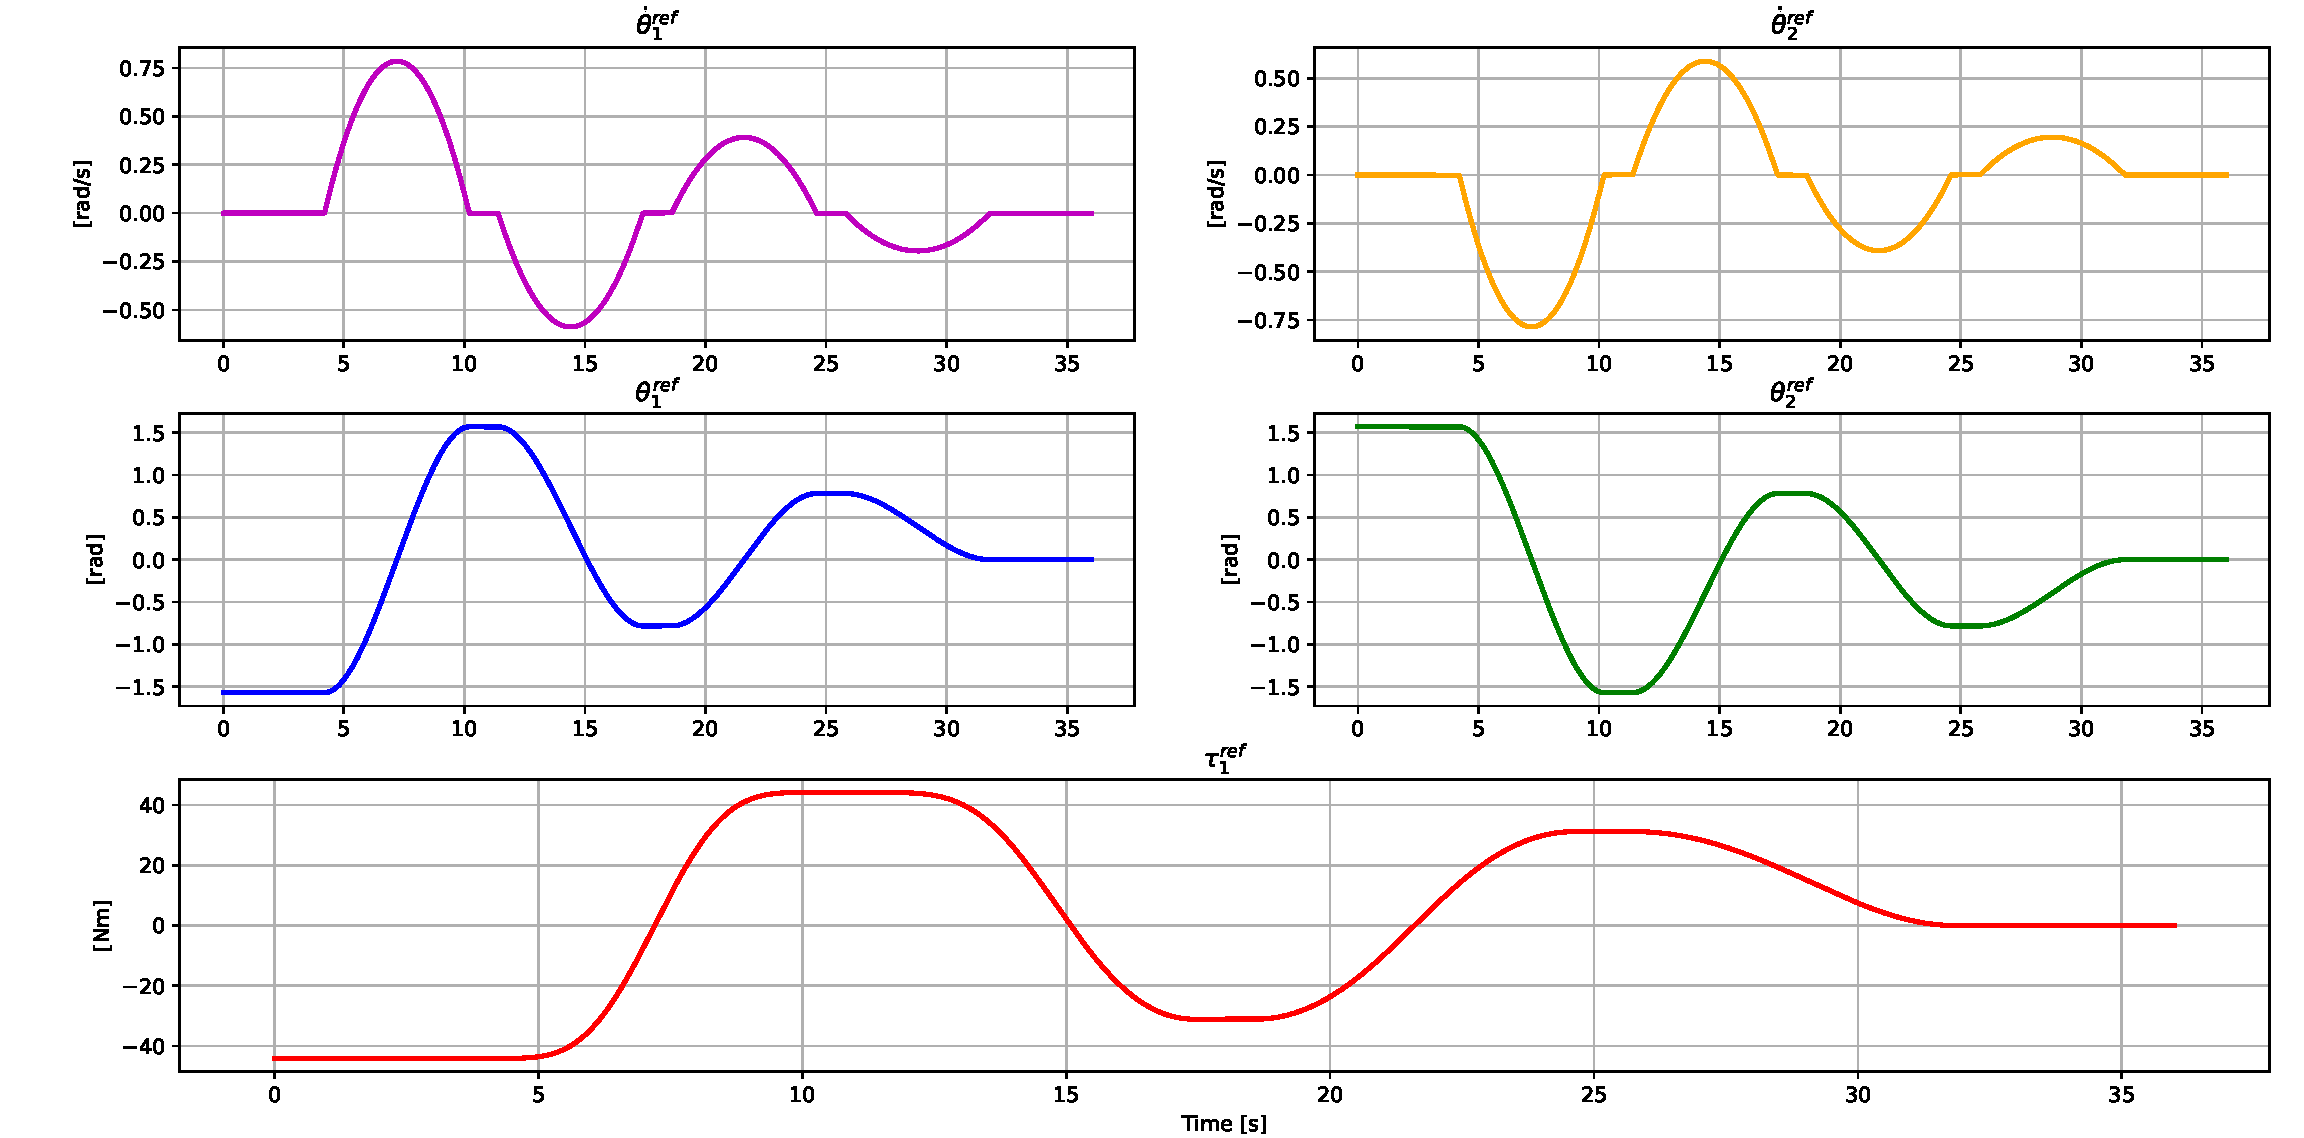
\includegraphics[width=1\linewidth]{img/2-task2/References.pdf}
    \caption{Smooth reference curve.}
    \label{fig:tau1-evolution}
\end{figure}

% - Explain the concept of quasi-static trajectories and their role in initialization.

More precisely, this is a quasi-static trajectory; it represents a gradual and steady evolution of the system's states, during which the system remains in or near equilibrium at all times. This approach ensures that dynamic effects, such as transients or inertia, are negligible, as the system has sufficient time to adjust to changes and maintain balance.

In the context of optimal control, quasi-static trajectories play an important role in the initialization process. They provide smooth and feasible transitions between equilibrium points, preventing abrupt changes that could lead to instability or infeasibility. By simplifying the dynamics and avoiding abrupt changes, they ensure stability, facilitate the computation of initial conditions, and improve the convergence of optimization algorithms.

\section{Improved Optimal Transition}
% - Extend the approach from Task 1 to refine the smoother trajectory.
In Task 2, the same optimal control problem is addressed as in Task 1, with the distinction that the reference curve from which the system starts is a smooth transition between equilibrium points. The cost function is defined in Equation (2.1) and the cost matrices are time-varying, with the following behavior.

\begin{figure}[htb]
    \centering
    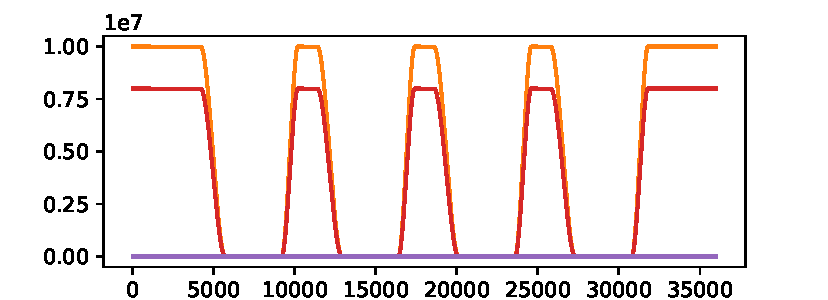
\includegraphics[width=1\linewidth]{img/2-task2/cost_evolution.pdf}
    \caption{Evolution of cost matrices.}
    \label{fig:dtheta2-evolution}
\end{figure}


% - Describe how LQR is used for generating a feasible initial guess.
\newpage
\section{Plots for Trajectory Generation (II)}
\begin{figure}[htb]
    \centering
    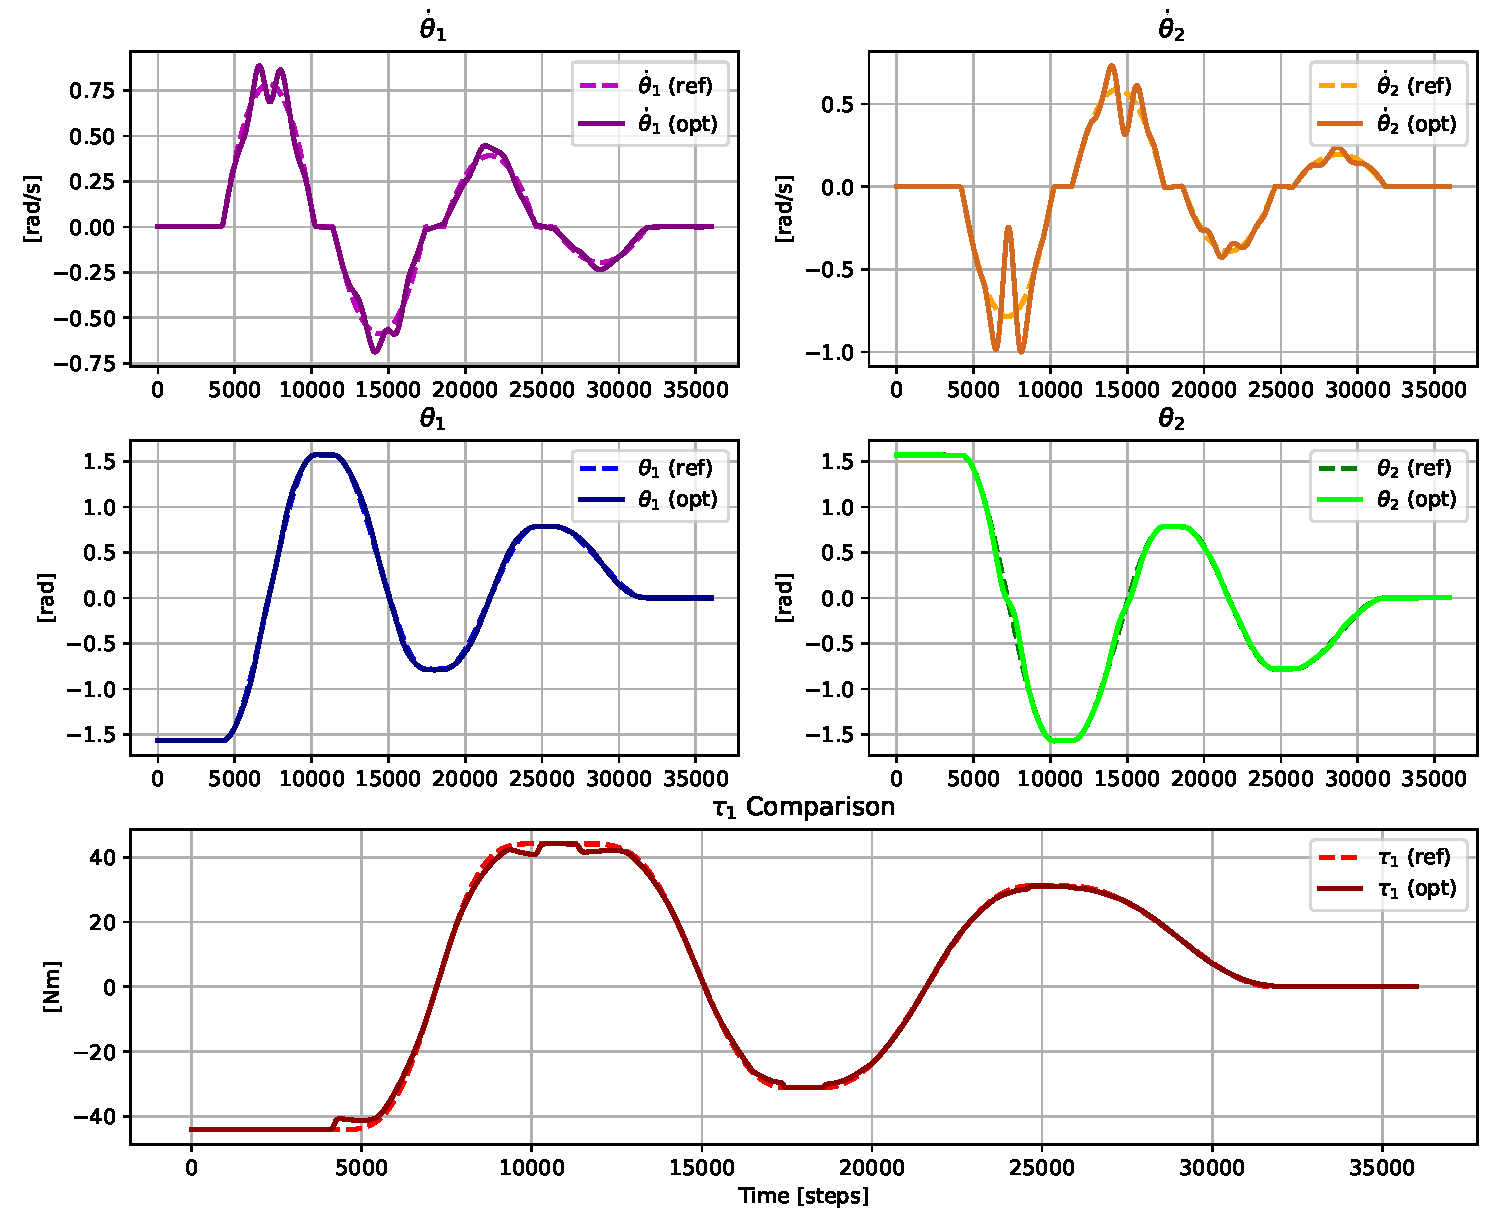
\includegraphics[width=1\linewidth]{img/2-task2/Residuals.pdf}
    \caption{Generated optimal trajectory given a smooth reference.} %do not forget to add \cite{} inside caption if it is noy your picture
    \label{fig:optimal-step}
\end{figure}

\begin{figure}[htb]
    \centering
    % First 3 images on the first page
    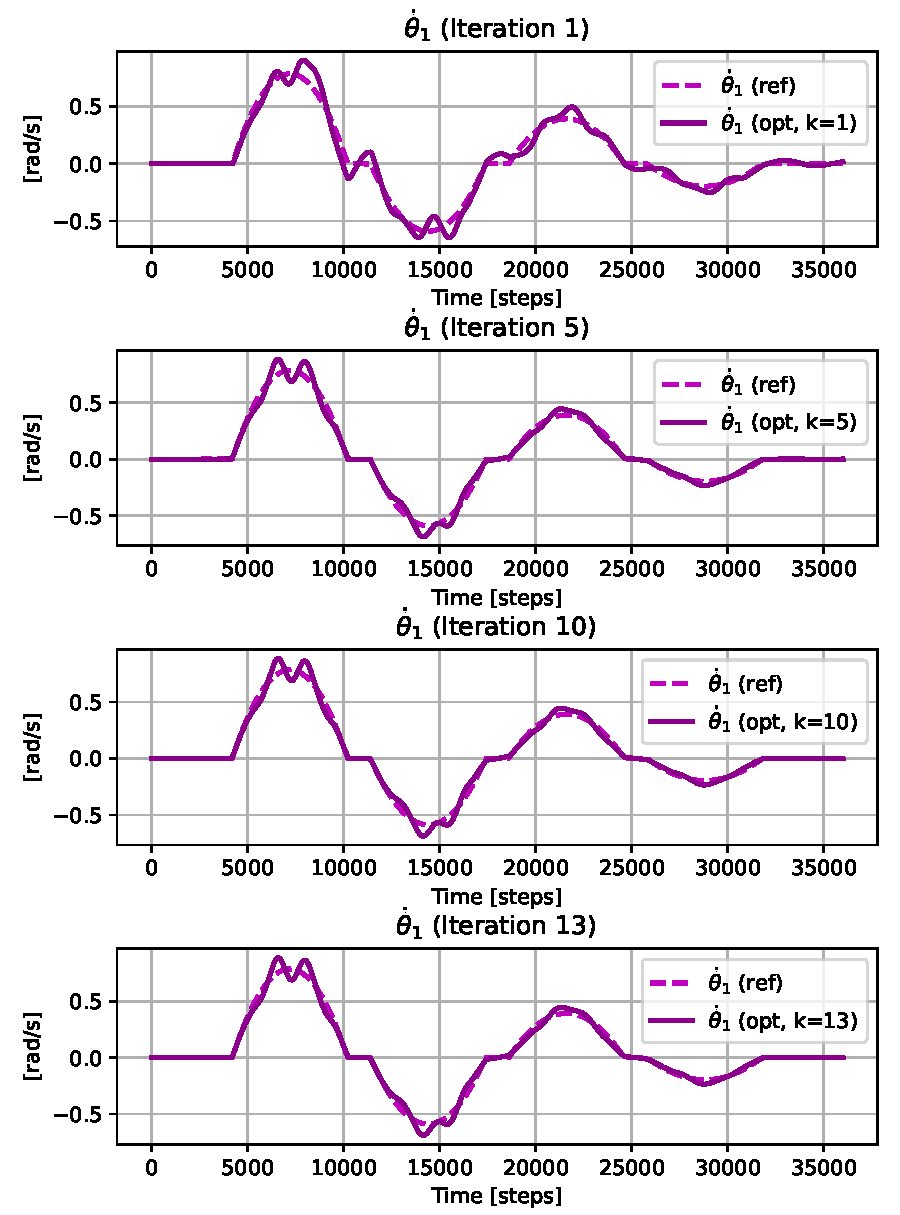
\includegraphics[width=1\linewidth]{img/2-task2/th1dot_evolution.pdf}
    \caption{Evolution of $d\theta_1$.}
    \label{fig:dtheta1-evolution}
\end{figure}
    
\begin{figure}[htb]
    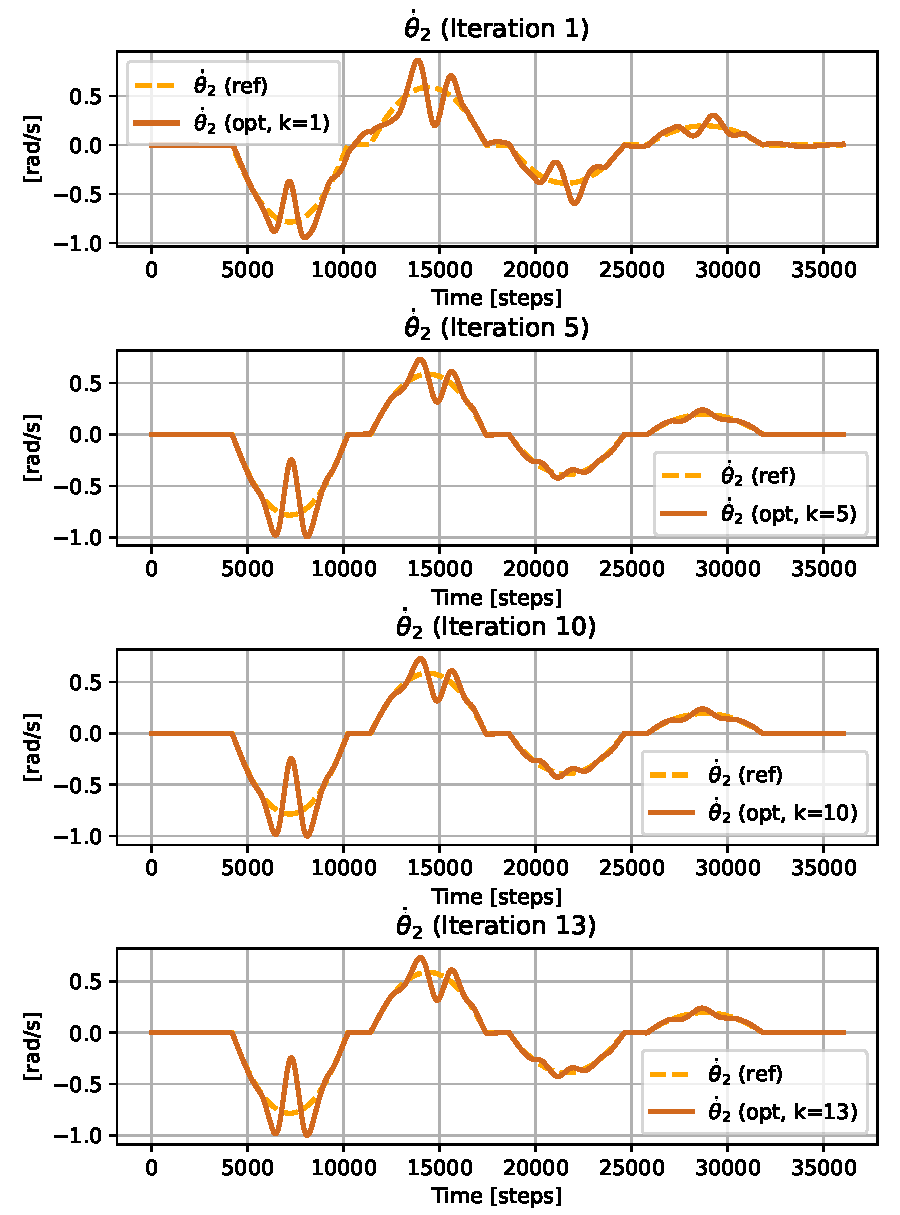
\includegraphics[width=1\linewidth]{img/2-task2/th2dot_evolution.pdf}
    \caption{Evolution of $d\theta_2$.}
    \label{fig:dtheta2-evolution}
\end{figure}

\begin{figure}[htb]
    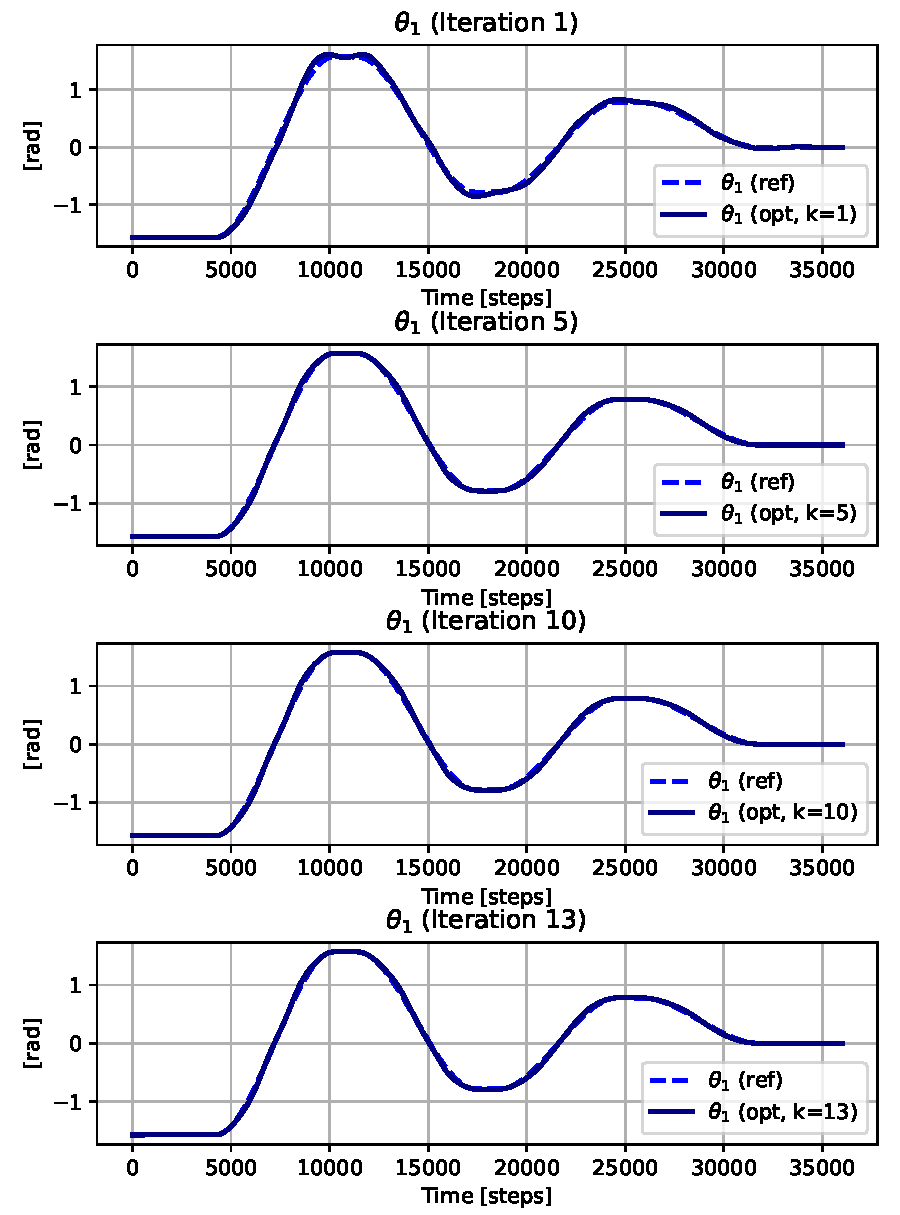
\includegraphics[width=1\linewidth]{img/2-task2/th1_evolution.pdf}
    \caption{Evolution of $\theta_1$.}
    \label{fig:theta1-evolution}
\end{figure}

\begin{figure}[htb]
    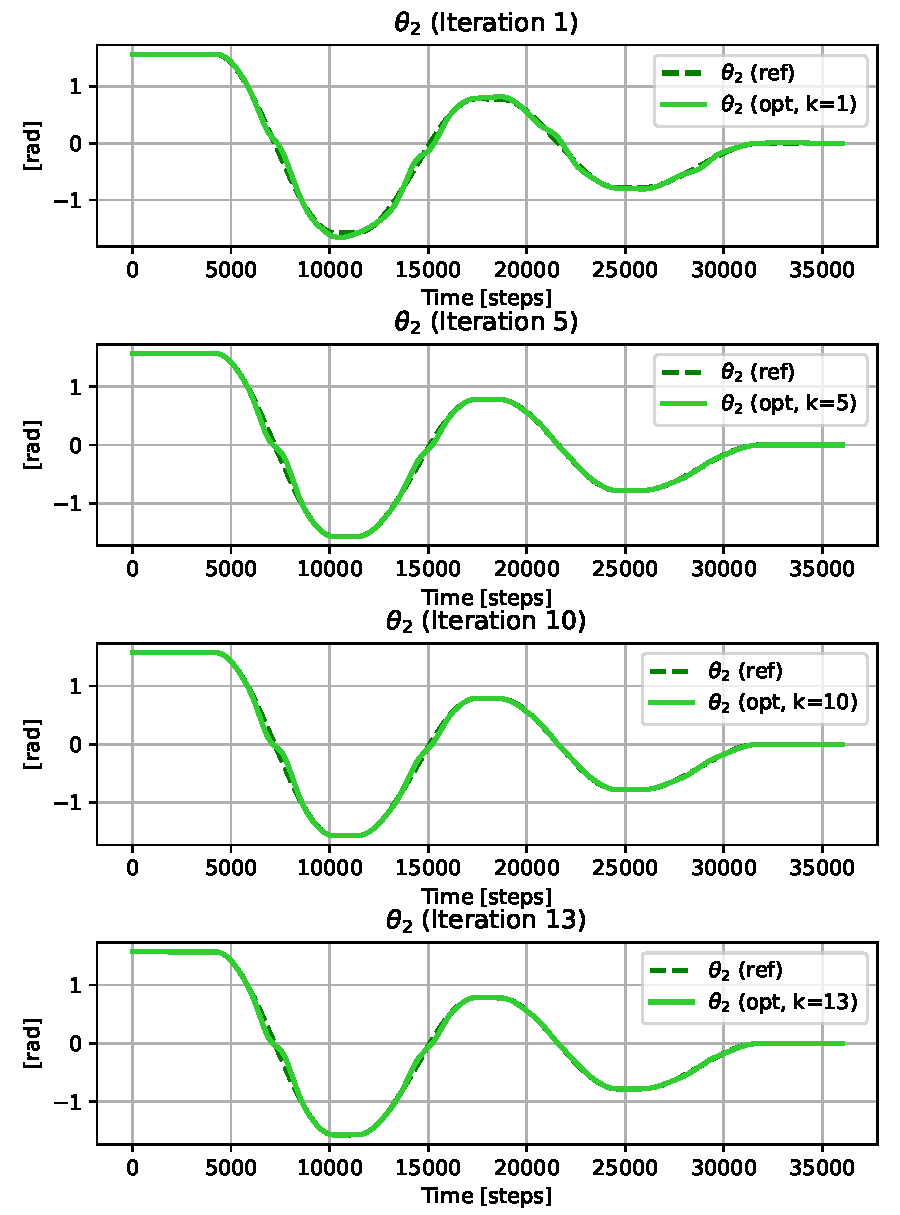
\includegraphics[width=1\linewidth]{img/2-task2/th2_evolution.pdf}
    \caption{Evolution of $\theta_2$.}
    \label{fig:theta2-evolution}
\end{figure}

\begin{figure}[htb]
    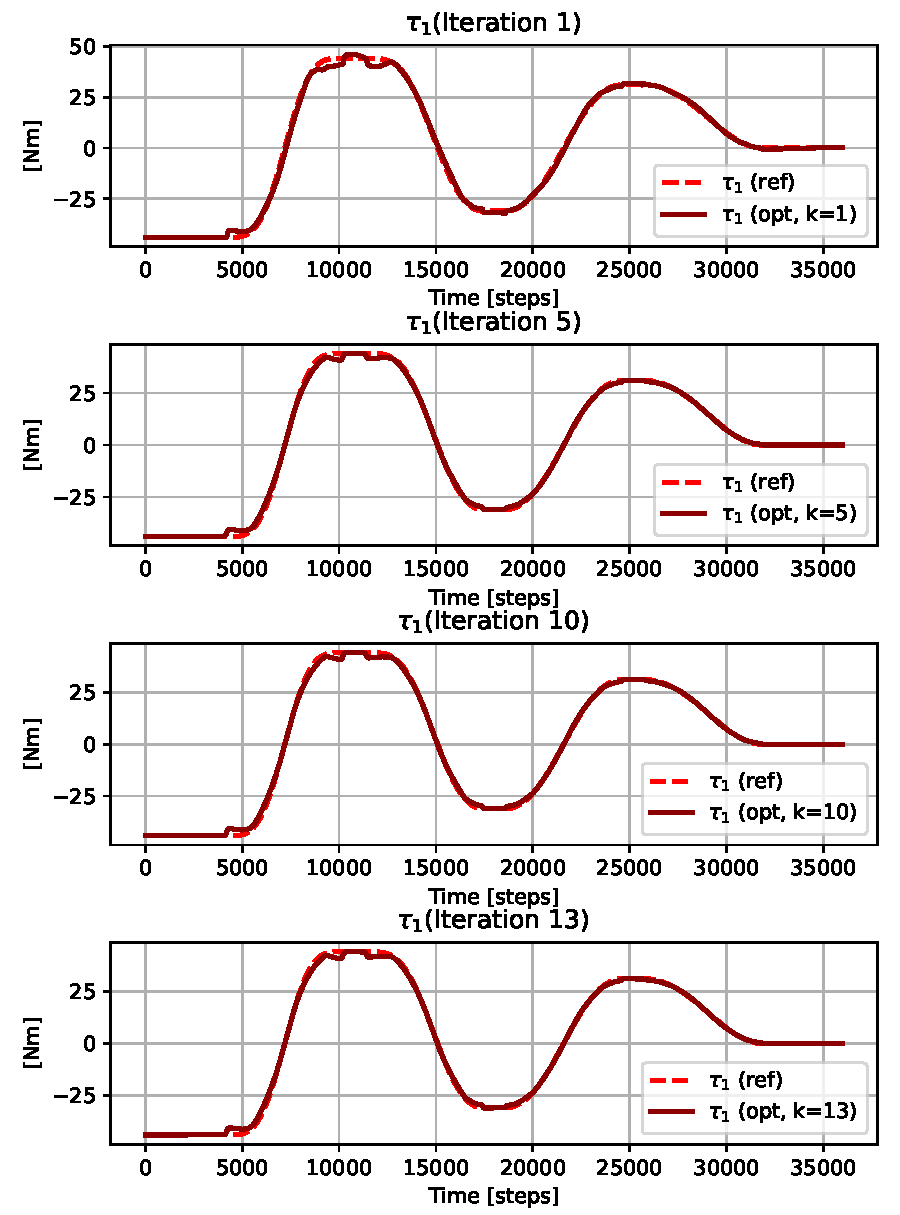
\includegraphics[width=1\linewidth]{img/2-task2/tau_evolution.pdf}
    \caption{Evolution of $\tau_1$.}
    \label{fig:tau1-evolution}
\end{figure}

\begin{figure}[htb]
    \centering
    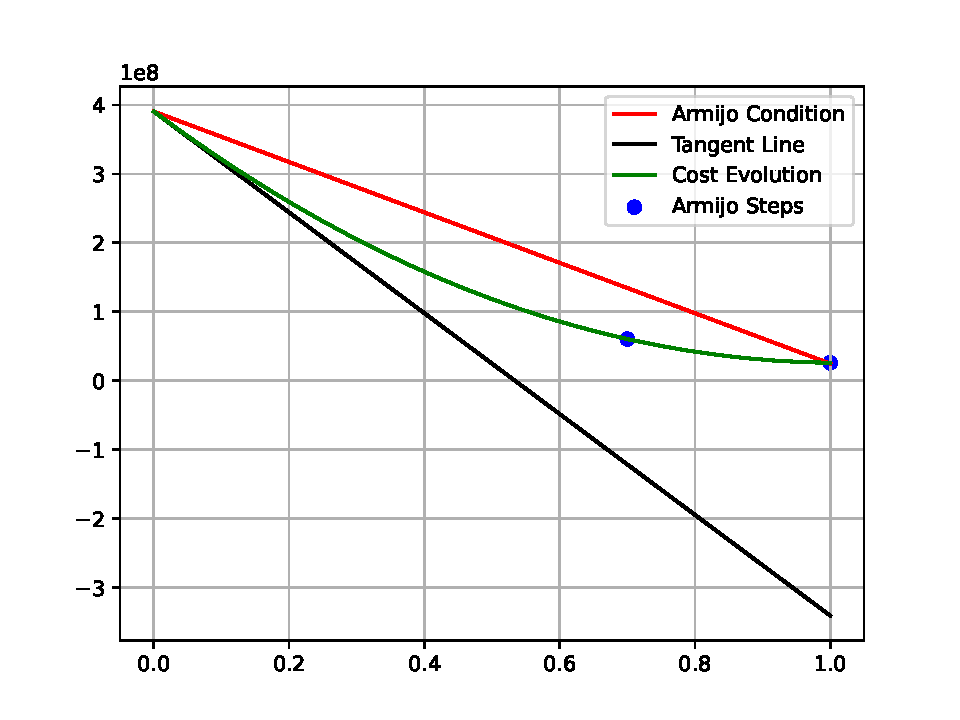
\includegraphics[width=1\linewidth]{img/2-task2/Armijo_iter_1.pdf}
    \caption{Armijo step-size selection: iteration 1}
    \label{fig:armijo1}
\end{figure}

\begin{figure}[htb]
    \centering
    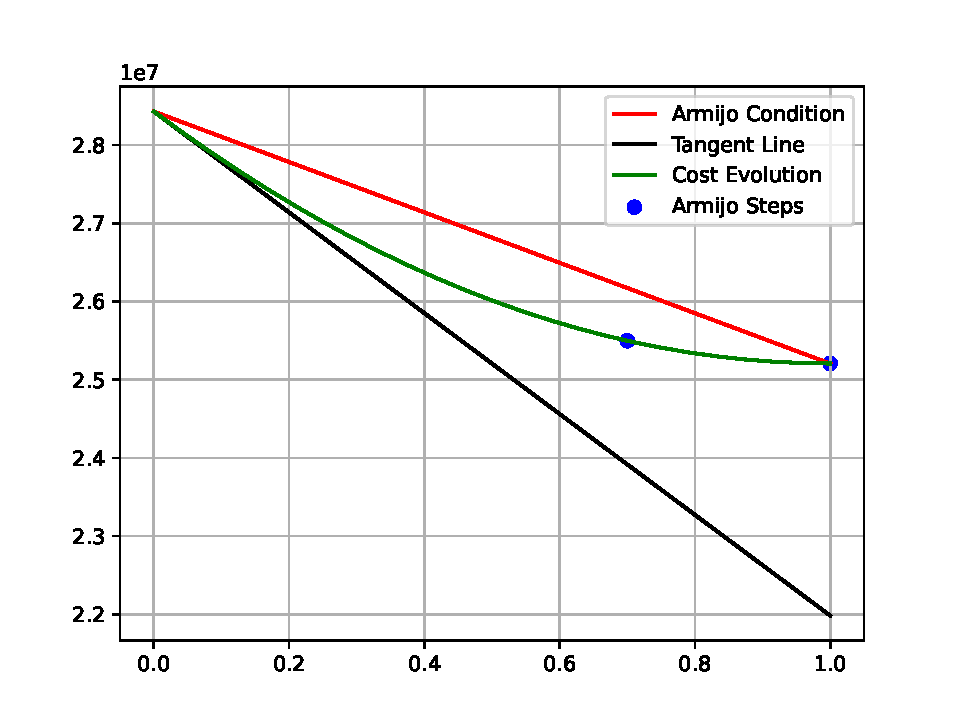
\includegraphics[width=1\linewidth]{img/2-task2/Armijo_iter_3.pdf}
    \caption{Armijo step-size selection: iteration 3}
    \label{fig:armijo1}
\end{figure}

\begin{figure}[htb]
    \centering
    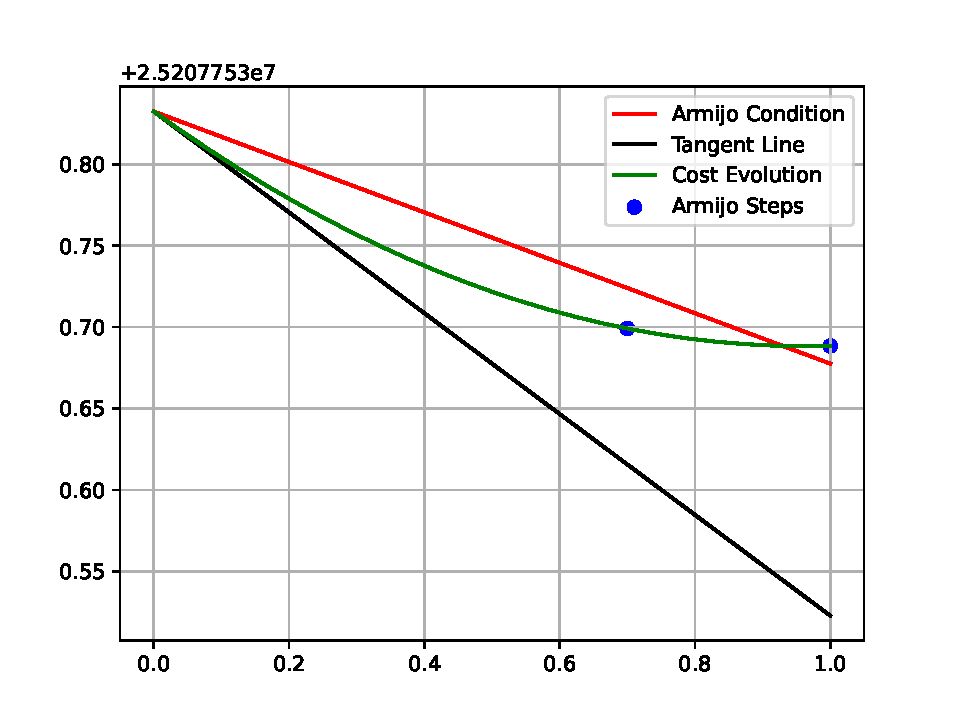
\includegraphics[width=1\linewidth]{img/2-task2/Armijo_iter_10.pdf}
    \caption{Armijo step-size selection: iteration 10}
    \label{fig:armijo1}
\end{figure}

\begin{figure}[htb]
    \centering
    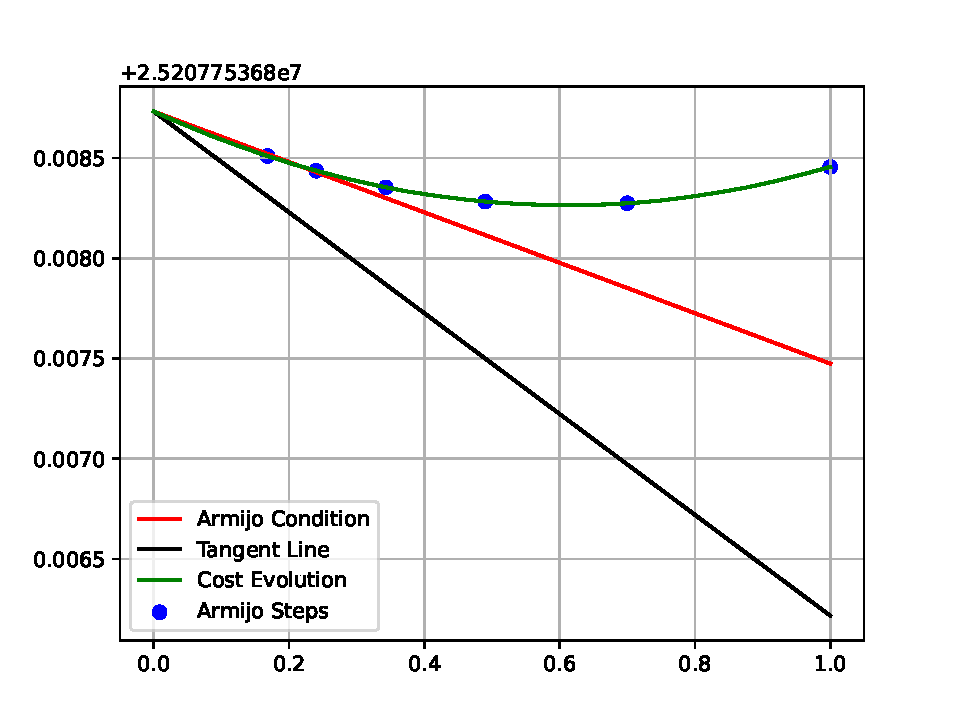
\includegraphics[width=1\linewidth]{img/2-task2/Armijo_iter_12.pdf}
    \caption{Armijo step-size selection: iteration: 12}
    \label{fig:armijo1}
\end{figure}
% - Required plots:
%   - Optimal trajectory vs. smooth desired curve.
%   - Intermediate trajectories and convergence trends (descent direction norms and costs).
\begin{figure}[htb]
    \centering
    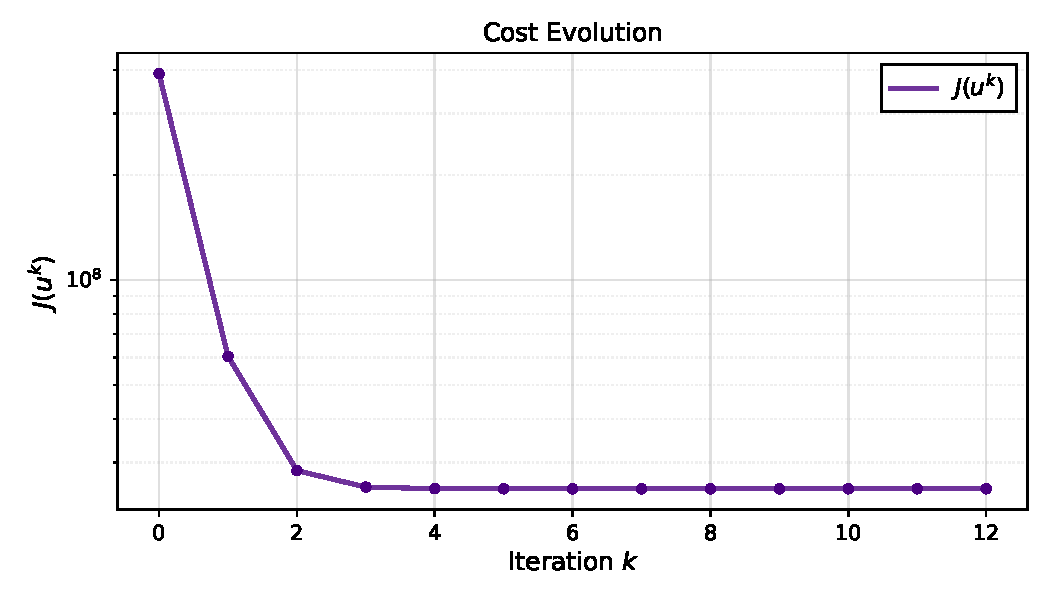
\includegraphics[width=1\linewidth]{img/2-task2/Cost_evolution.pdf}
    \caption{Cost evolution}
    \label{fig:armijo1}
\end{figure}

\begin{figure}[htb]
    \centering
    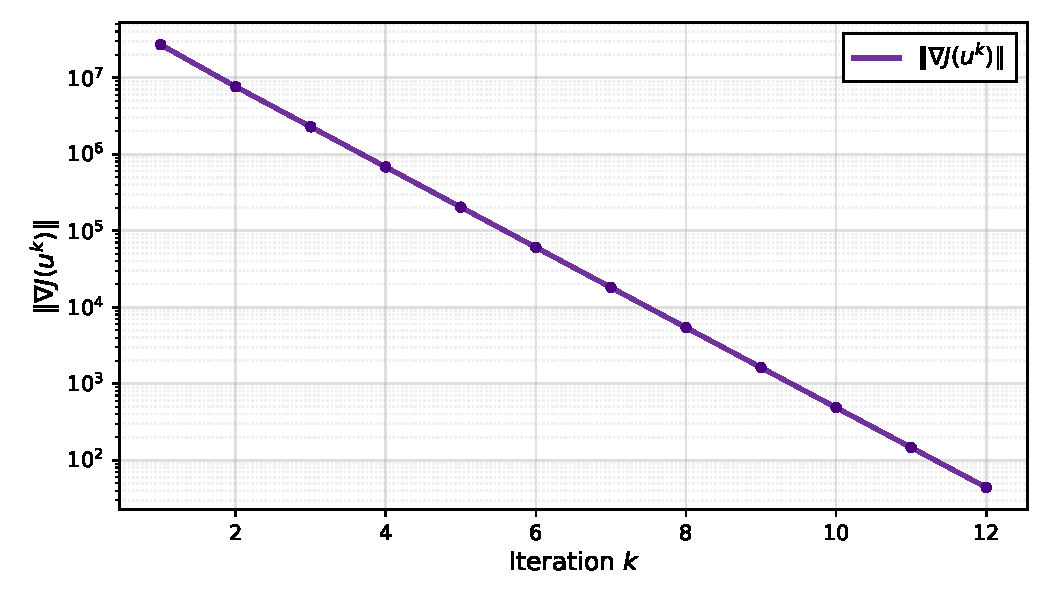
\includegraphics[width=1\linewidth]{img/2-task2/grad_J_norm.pdf}
    \caption{Cost gradient norm evolution}
    \label{fig:armijo1}
\end{figure}

\begin{figure}[htb]
    \centering
    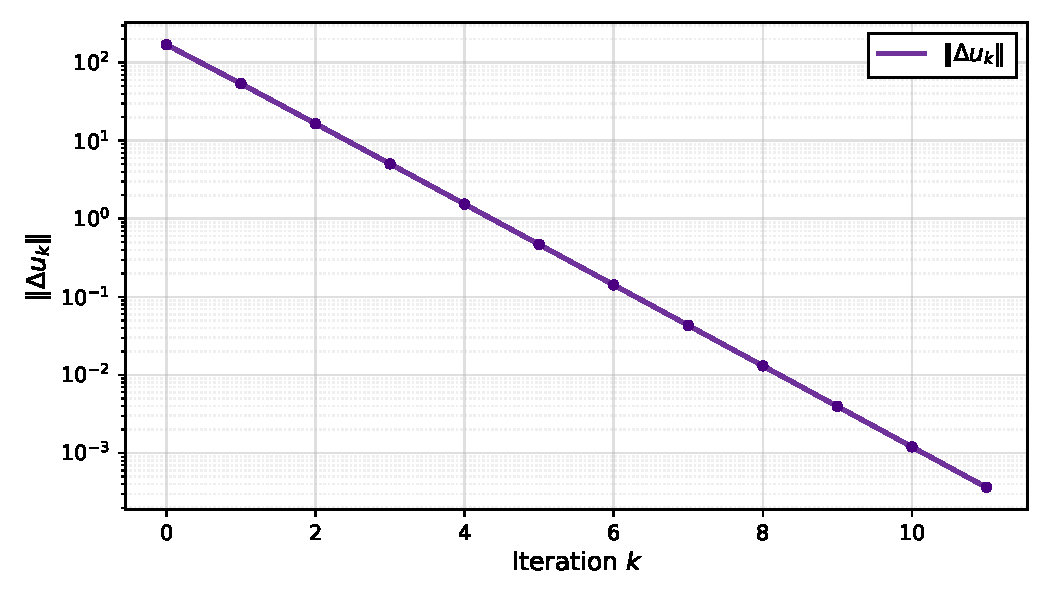
\includegraphics[width=1\linewidth]{img/2-task2/delta_u_norm.pdf}
    \caption{Evolution of $||\Delta u_k||$}
    \label{fig:armijo1}
\end{figure}

\clearpage


\newpage
\section{Constant Cost Matrices Scenario}

The following cost matrices have been adopted:
\begin{equation}
Q_t = Q_T
=
\begin{bmatrix}
    10 & 0 & 0 & 0\\
    0 & 10 & 0 & 0\\
    0 & 0 & 10 & 0\\
    0 & 0 & 0 & 10\\
\end{bmatrix}
\label{eq:CosntantQ}
\end{equation}

\begin{equation}
R_t = 
\begin{bmatrix}
    0.3 & 0 & 0 & 0\\
    0 & 0.3 & 0 & 0\\
    0 & 0 & 0.3 & 0\\
    0 & 0 & 0 & 0.3\\
\end{bmatrix}
\label{eq:ConstantR}
\end{equation}
\newline
Here, a summary of the results is presented.\newline
The performances are obviously worse than the ones presented before.

\begin{figure}[htb]
    \centering
    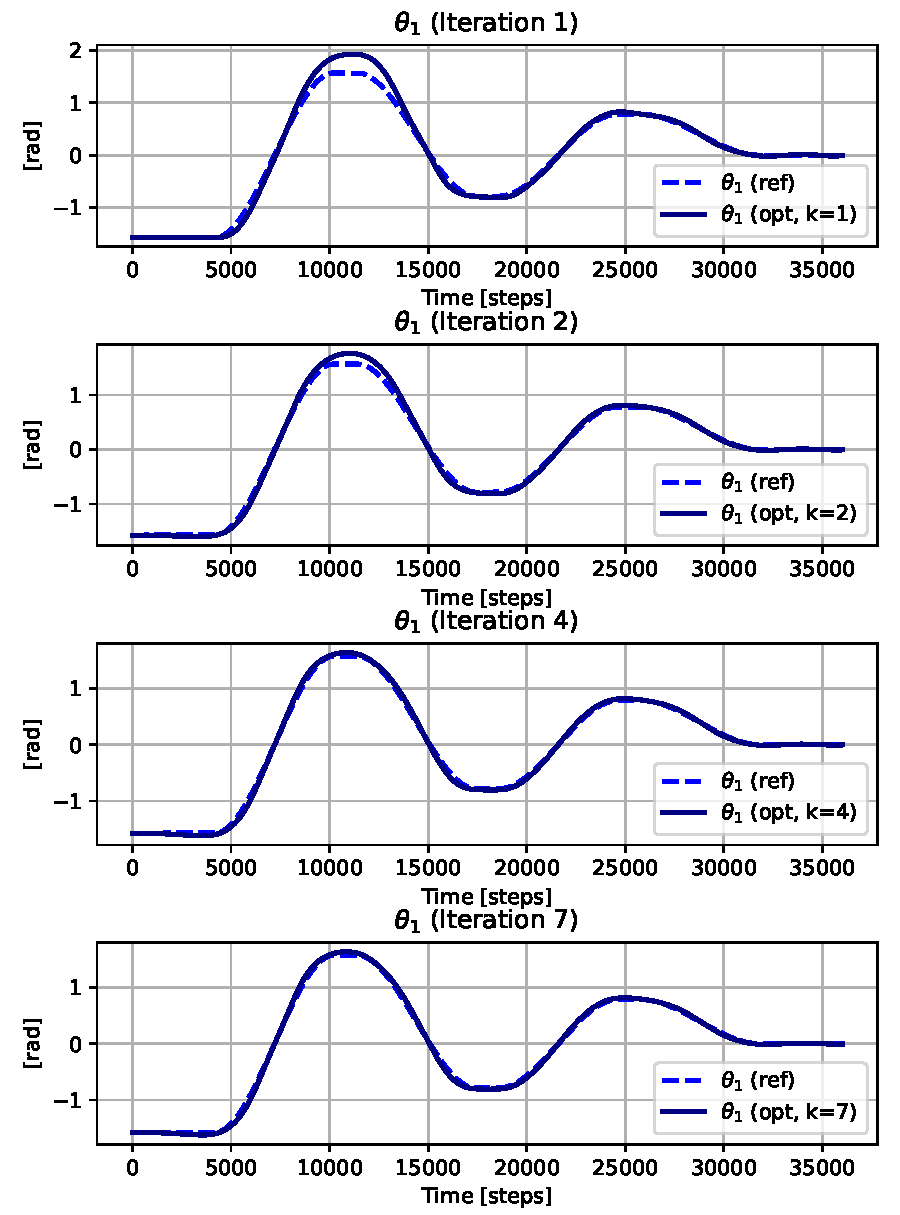
\includegraphics[width=1\linewidth]{img/2-task2/t1_const.pdf}
    \caption{Evolution of $\theta_1$ with constant Cost Matrices.}
    \label{fig:th1const_}
\end{figure}

\begin{figure}[htb]
    \centering
    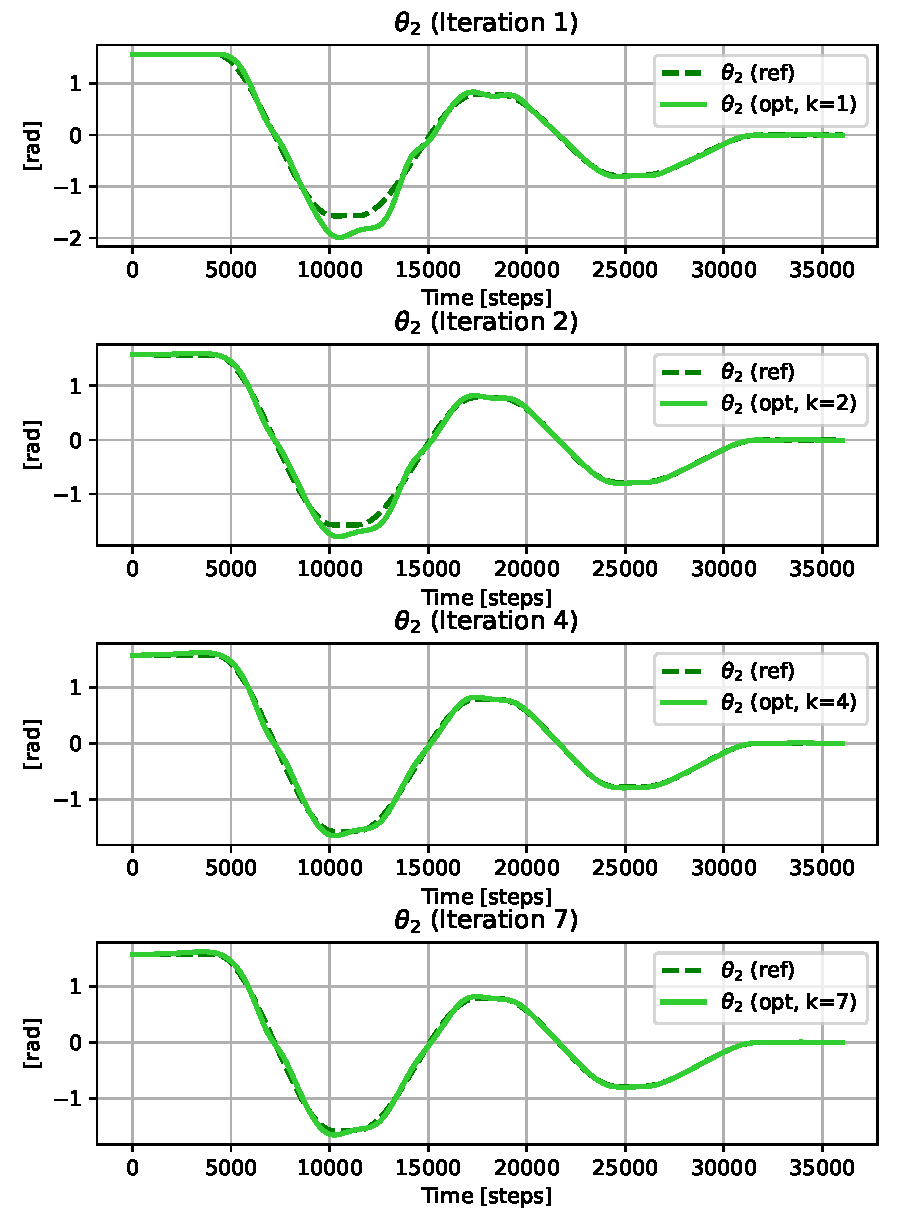
\includegraphics[width=1\linewidth]{img/2-task2/t2_const.pdf}
    \caption{Evolution of $\theta_2$ with constant Cost Matrices.}
    \label{fig:th2const_}
\end{figure}

\clearpage

\begin{figure}[htb]
    \centering
    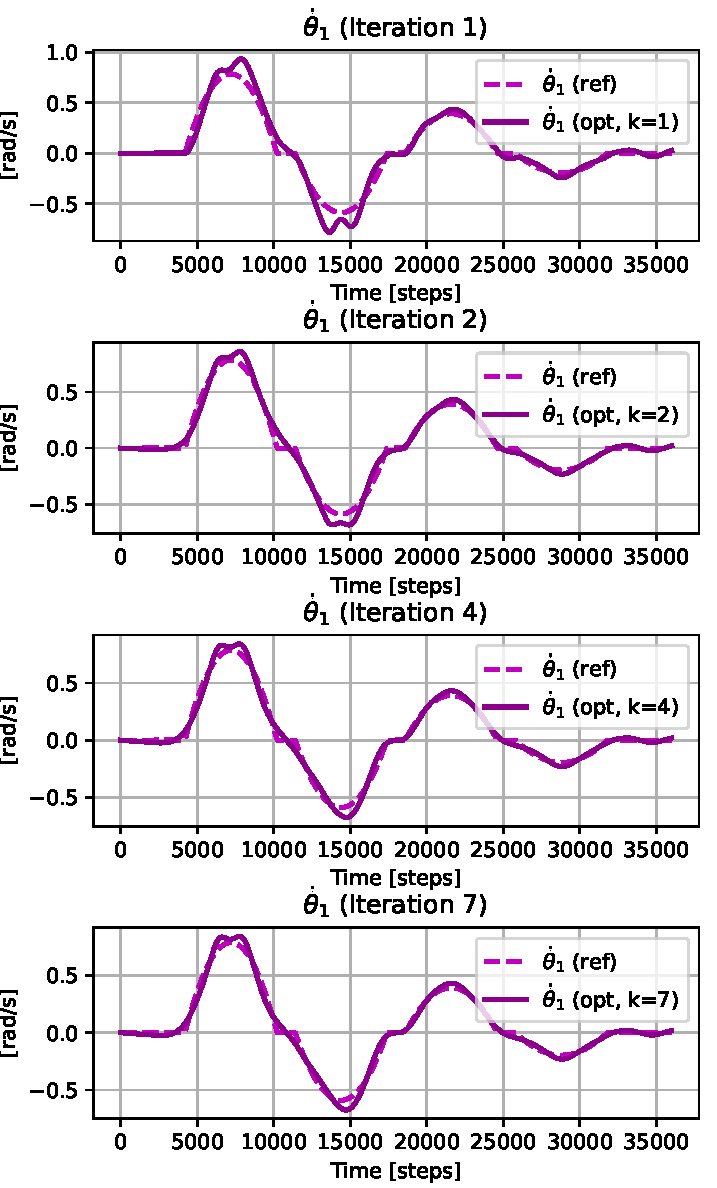
\includegraphics[width=0.9\linewidth]{img/2-task2/t1d_const.pdf}
    \caption{Evolution of $\dot{\theta_1}$ with constant Cost Matrices.}
    \label{fig:th1dot_const_}
\end{figure}

\begin{figure}[htb]
    \centering
    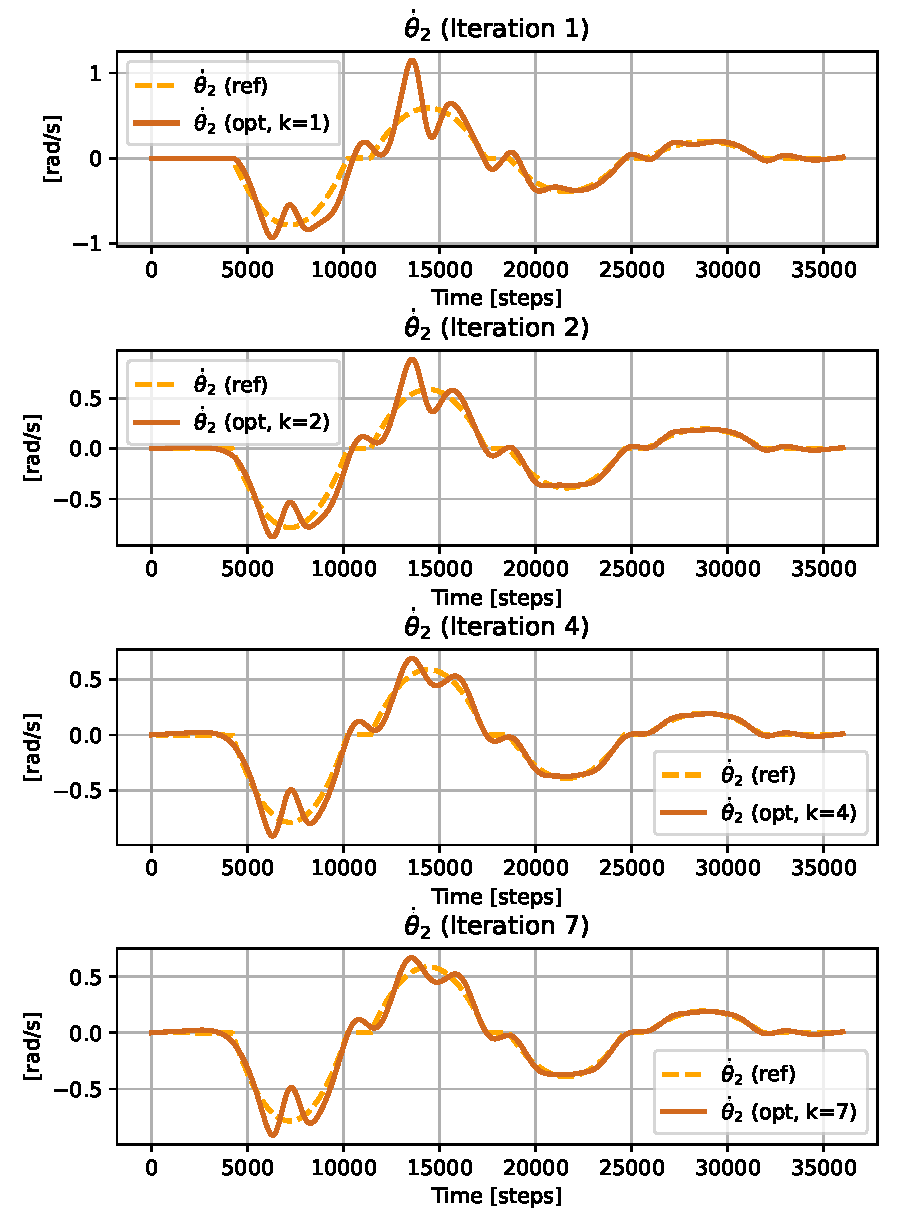
\includegraphics[width=1\linewidth]{img/2-task2/t2d_const.pdf}
    \caption{Evolution of $\dot{\theta_2}$ with constant Cost Matrices.}
    \label{fig:th2_const_}
\end{figure}

\begin{figure}[htb]
    \centering
    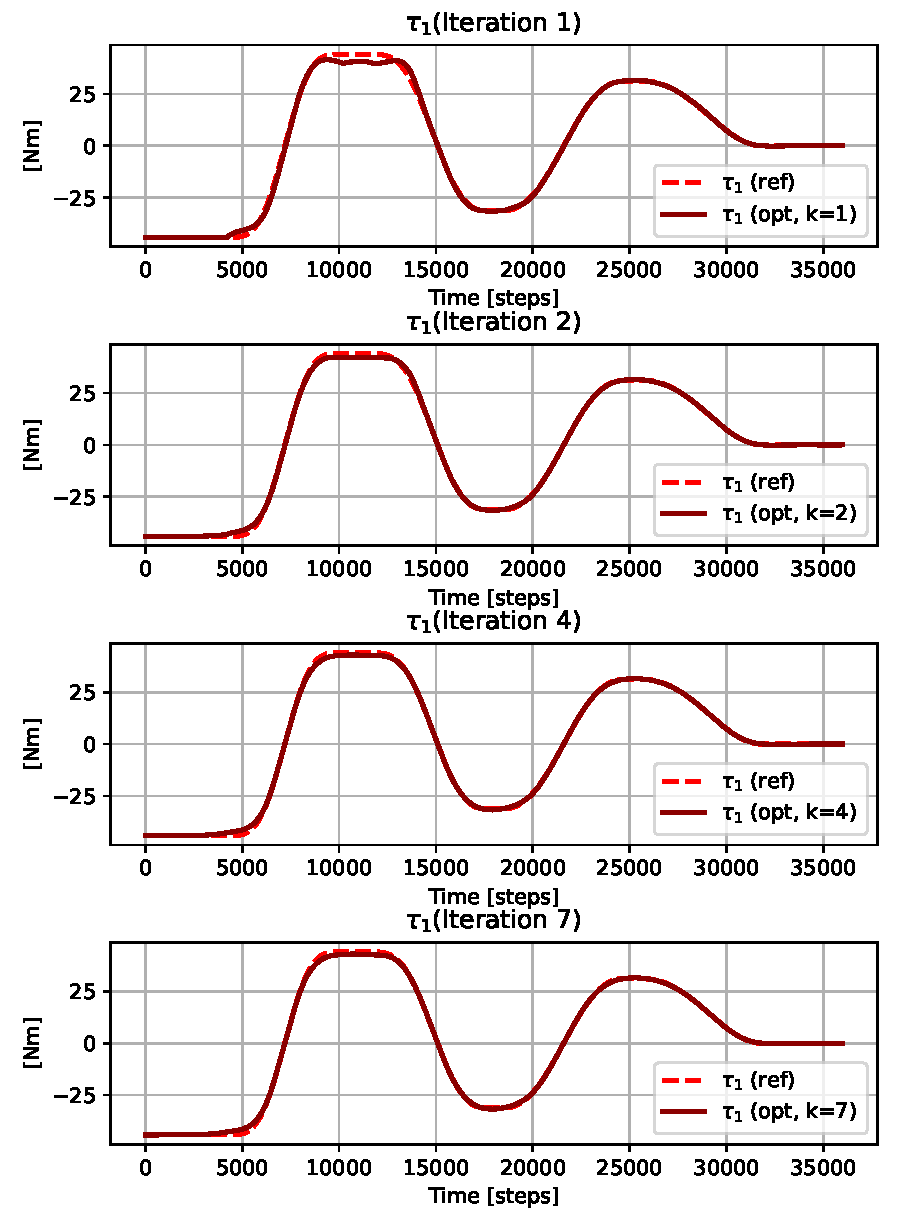
\includegraphics[width=1\linewidth]{img/2-task2/tau_const.pdf}
    \caption{Evolution of $\tau$ with constant Cost Matrices.}
    \label{fig:tau_const_}
\end{figure}

\begin{figure}[htb]
    \centering
    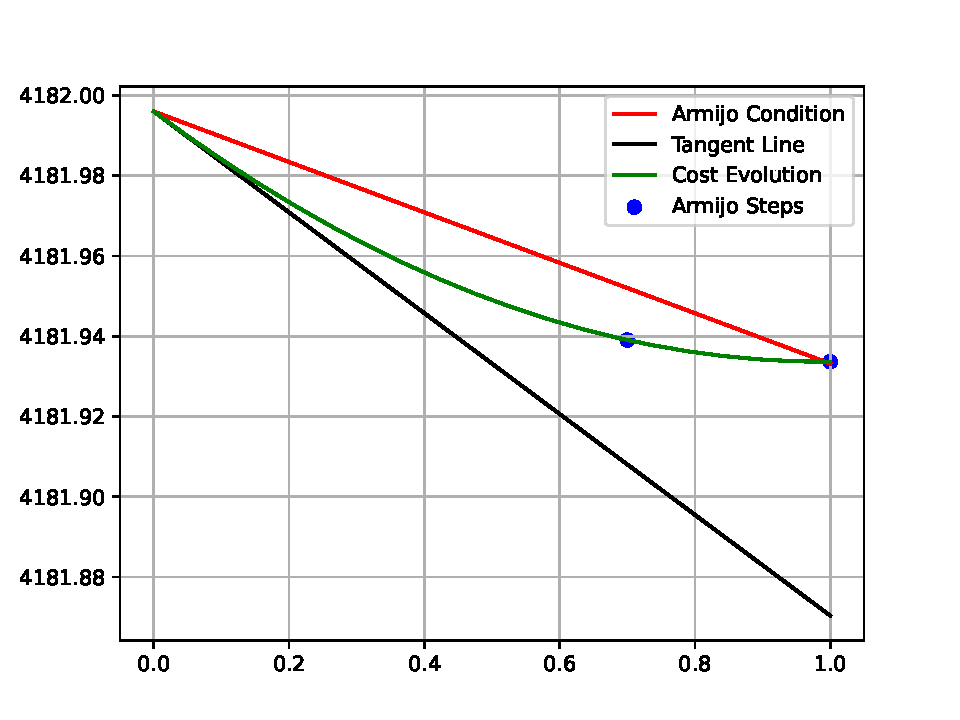
\includegraphics[width=1\linewidth]{img/2-task2/Armijo_Last_Step_const.pdf}
    \caption{Armijo step-size selection: last iteration.}
    \label{fig:lastiter}
\end{figure}


\clearpage

\begin{figure}[htb]
    \centering
    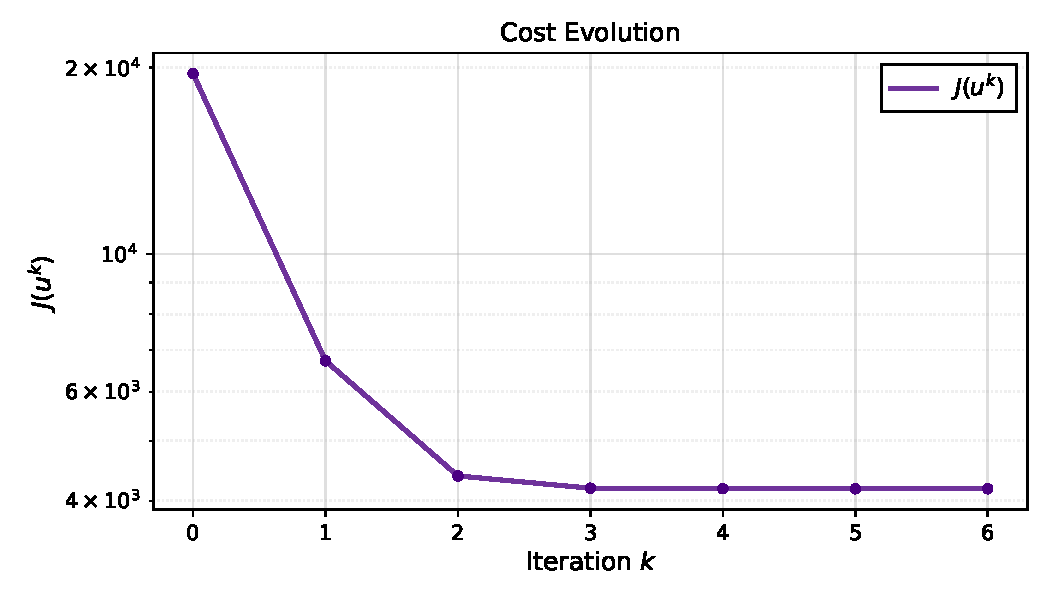
\includegraphics[width=1\linewidth]{img/2-task2/cost_const.pdf}
    \caption{Evolution of cost function with constant Cost Matrices.}
    \label{fig:J_const}
\end{figure}

\begin{figure}[htb]
    \centering
    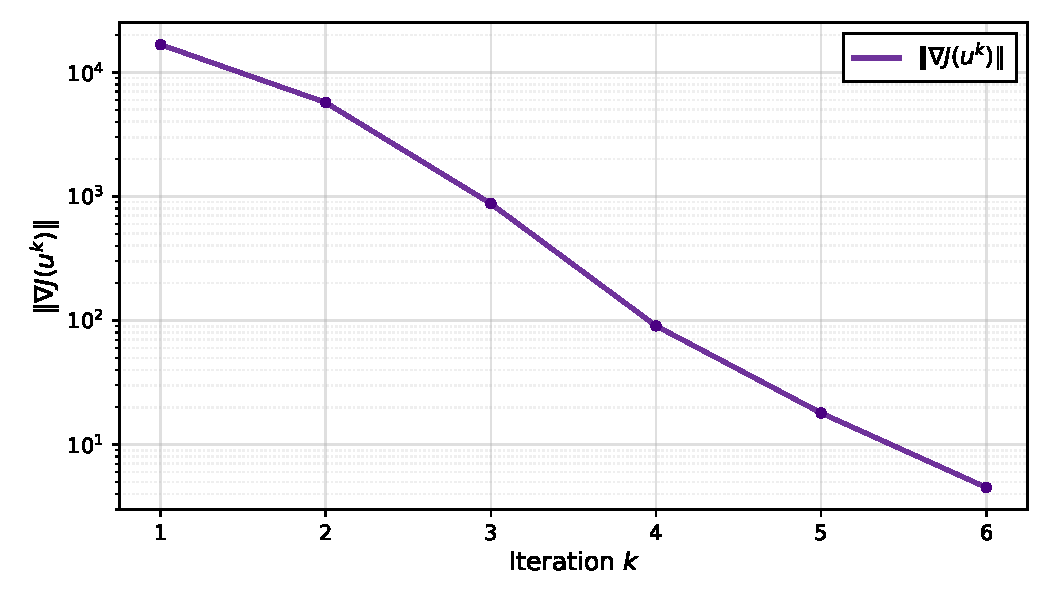
\includegraphics[width=1\linewidth]{img/2-task2/gradJ_const.pdf}
    \caption{Evolution of $||\nabla J(u)||$ with constant Cost Matrices.}
    \label{fig:NormJ_const}
\end{figure}

\begin{figure}[htb]
    \centering
    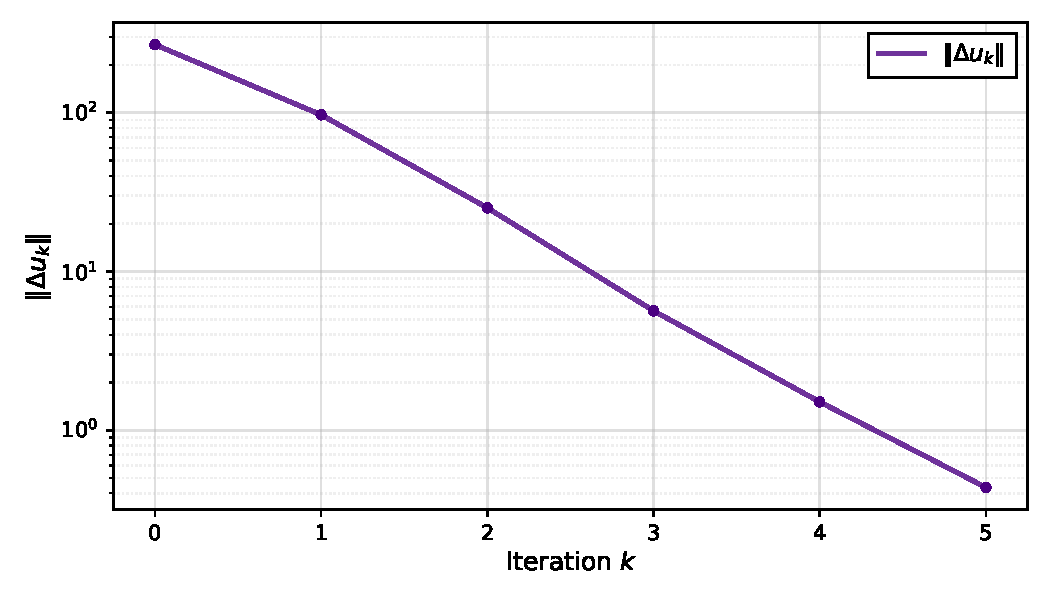
\includegraphics[width=1\linewidth]{img/2-task2/delta_u_const.pdf}
    \caption{Evolution of $||\Delta u_k||$ with constant Cost Matrices.}
    \label{fig:normdu_const}
\end{figure}
